\chapter{Thermodynamics of the expanding universe}
\label{chapter:thermodynamicsofearlyuniverse}

In this chapter, our objective is to understand the evolution of the early universe, so we will make a brief review of the thermodynamics in the equilibrium of the early universe, following \cite{kolb}.

We are able to predict how the universe behaved due to the Cosmic Microwave Background (CMB) being approximately equal to the spectra of a black body, so we assume that in the primordial universe the particles from the SM are in equilibrium.

\section{Thermodynamics in equilibrium}
The number density, $n$, energy density, $\rho$, and the pressure, $P$ of a gas of particles with a degree of freedom, $g$, distinguish the thermodynamic properties of the gas and are defined as a function of the distribution function $f(\vec{p},t)$:
\begin{equation}
	\label{eqn:3.1}
	n(t)\equiv\frac{g}{(2\pi)^3}\int f(\vec{p},t) d\vec{p}\,,
\end{equation}
\begin{equation}
	\label{eqn:3.2}
	\rho(t)\equiv\frac{g}{(2\pi)^3}\int E(\vec{p})f(\vec{p},t) d\vec{p}\,,
\end{equation} 
\begin{equation}
	\label{eqn:3.3}
	P(t)\equiv\frac{g}{(2\pi)^3}\int \frac{p^2}{3E}f(\vec{p},t) d\vec{p}\,,
\end{equation}  
where $\vec{p}=(p_x,p_y,p_z)$, $d\vec{p}\equiv dp_xdp_ydp_z$ and E=$\sqrt{p^2+m^2}$. The phase pace equilibrium distribution function for a particle $i$ will be given by one of the three following distributions
\begin{equation}
	f_i^{eq} = \left\{ 
	\begin{array}{lll}
		\frac{1}{e^{(E_i-\mu_i)/T}+1}\,, \quad\textrm{Fermi-Dirac}\,,\\
		\frac{1}{e^{(E_i-\mu_i)/T}-1}\,, \quad\textrm{Bose-Einstein}\,,\\
		e^{-(E_i-\mu_i)/T}\,, \quad \textrm{Maxwell-Boltzmann}\,,	
	\end{array}
	\right.
\end{equation}
where $E_i$ and $\mu_i$ is the energy and chemical potential of the particle $i$, respectively. The Fermi-Dirac (Bose-Einstein) statistic refers to particles with half-integer (integer) spin.

Using spherical symmetry we can simplify, $d\vec{p}=4\pi p^2dp,$ we can now rewrite the Equations (\ref{eqn:3.1}), (\ref{eqn:3.2}) and (\ref{eqn:3.3}) in function of the energy, $E$, given as
\begin{equation}
	\label{eqn:3.5}
	n_R=\frac{g}{2\pi^2}\int_{m}^{\infty} \frac{(E^2-m^2)^{1/2}}{e^{(E-\mu)/T}\pm 1}dE\,,
\end{equation}
\begin{equation}
	\label{eqn:3.6}
	\rho_R=\frac{g}{2\pi^2}\int_{m}^{\infty} \frac{(E^2-m^2)^{1/2}}{e^{(E-\mu)/T}\pm 1}E^2dE\,,
\end{equation} 
\begin{equation}
	\label{eqn:3.7}
	P_R=\frac{g}{6\pi^2}\int_{m}^{\infty} \frac{(E^2-m^2)^{3/2}}{e^{(E-\mu)/T}\pm 1}dE\,,
\end{equation}
where "R"\ refers to radiation, the inferior limit of the integral refers to the lowest energy a particle can have, which is its mass, $m$.

Let's take a look at a generalized solution for the Fermi-Dirac and Bose-Einstein distributions, when we take into account that the mass of the particle is so low such that, $m \simeq 0$, we get
\begin{equation}
	\nonumber
	\int_{m}^{\infty} \frac{(E^2-m^2)^s}{e^{(E-\mu)/T}\pm 1}dE =  	\int_{0}^{\infty}\frac{E^s}{e^{\frac{E-\mu_i}{T}}\pm 1}dE\,,
\end{equation}
by making $k=\frac{E}{T}$ and $\mu=\frac{\mu_i}{T}$, we get \cite{fermi}\cite{bose}
\begin{equation}
	\label{eqn:3.8}
	\int_{0}^{\infty}\frac{E^s}{e^{\frac{E-\mu_i}{T}}\pm 1}dE =\int_{0}^{\infty}\frac{(Tk)^s}{e^{k-\mu}\pm 1}Tdk=T^{s+1}\int_{0}^{\infty}\frac{k^s}{e^{k-\mu}\pm 1}dk=\mp T^{s+1} \Gamma(s+1)Li_{1+s}(\mp e^\mu)\,,
\end{equation}
where the polylogarithm or Jonquière's function and the Gamma function, are respectively defined by \cite{poly}
\begin{equation}
	\label{eqn:3.9}
	Li_n(z)\equiv\sum\limits_{k=1}^\infty \frac{z^k}{k^n} \quad \textrm{and} \quad \Gamma(s+1)=\int_{0}^{\infty} e^{-x}x^s dx=s!\,.
\end{equation}

At the ultra-relativistic limit (radiation), $T\gg m,\mu_i$. We can simplify $\mu=\mu_i/T \simeq 0$ and so the polylogarithm function in \autoref{eqn:3.8} can be simplified into
\begin{equation}
	\label{eqn:3.10}
	Li_{s+1}(\mp 1)=\sum\limits_{k=1}^{\infty}\frac{(\mp1)^k}{k^{s+1}}\,,
\end{equation}
now if we take a look at the solution of the following sum
\begin{equation}
	\label{eqn:3.11}
	\sum\limits_{k=1}^{\infty}\frac{(-1)^{k+1}}{k^s}=(1-2^{-s})\zeta(s+1)\,,
\end{equation}
where $\zeta(s)$ the Riemann zeta function, defined by
\begin{equation}
	\label{eqn:3.12}
	\zeta(s)=\sum\limits_{k=1}^{\infty}\frac{1}{k^s}\,,
\end{equation}
using the solutions in Equations (\ref{eqn:3.11}) and (\ref{eqn:3.12}) the generalized solution for ultra-relativistic particles, in \autoref{eqn:3.8}, gets reduced to 
\begin{equation}
	\int_{0}^{\infty}\frac{E^s}{e^{\frac{E-\mu_i}{T}}\pm 1}dE=\left\{ \begin{array}{c}
		T^{s+1}(1-2^{-s})\zeta(s+1)s!\,, \quad \textrm{Fermi-Dirac}\,, \\
		T^{s+1}\zeta(s+1)s!\,, \quad \textrm{Bose-Einstein}\,,	
	\end{array}\right.\,.
\end{equation}
Now we can easily integrate the Equations (\ref{eqn:3.5}), (\ref{eqn:3.6}) and (\ref{eqn:3.7}), knowing that $\zeta(4)=\pi^4/90$ to
\begin{equation}
	\label{eqn:3.14}
	n_{\textrm{R}}=\frac{g}{2\pi^2}\int_{0}^{\infty} \frac{E}{e^{E/T}\pm1}dE=\frac{g}{\pi^2}T^3\zeta(3)\left\{ \begin{array}{c}
		3/4\,, \quad \textrm{Fermi-Dirac}\,, \\
		1\,, \quad \textrm{Bose-Einstein}\,,
	\end{array}\right.
\end{equation}
\begin{equation}
	\label{eqn:3.15}
	\rho_{\textrm{R}}=\frac{g}{2\pi^2}\int_{0}^{\infty} \frac{E^3}{e^{E/T}\pm1}dE=g\frac{\pi^2}{30}T^4\left\{ \begin{array}{c}
		7/8\,,\quad \textrm{Fermi-Dirac}\,, \\
		1\,, \quad \textrm{Bose-Einstein}\,,
	\end{array}\right.
\end{equation} 
\begin{equation}
	\label{eqn:3.16}
	P_{\textrm{R}}=\frac{g}{6\pi^2}\int_{0}^{\infty} \frac{E^3}{e^{E/T}\pm1}dE=\frac{1}{3}\rho_{\textrm{R}}\,,
\end{equation}  
where the + and - refers respectively to the Fermi-Dirac and Bose-Einstein distributions.

Now let's take a look at the non-relativistic limit (matter), $T \ll m,\mu$, which follows the Maxwell-Boltzmann distribution, we can rewrite the Equations (\ref{eqn:3.1}), (\ref{eqn:3.2}) and (\ref{eqn:3.3}) in function of the momentum, $p$, given as

\begin{equation}
	\label{eqn:3.17}
	n_{\textrm{M}}\equiv\frac{g}{(2\pi)^3}\int e^{-\frac{(E-\mu)}{T}} d\vec{p}\,,
\end{equation}
\begin{equation}
	\label{eqn:3.18}
	\rho_{\textrm{M}}\equiv\frac{g}{(2\pi)^3}\int E(\vec{p})e^{-\frac{(E-\mu)}{T}} d\vec{p}\,,
\end{equation} 
\begin{equation}
	\label{eqn:3.19}
	P_{\textrm{M}}\equiv\frac{g}{(2\pi)^3}\int \frac{p^2}{3E}e^{-\frac{(E-\mu)}{T}} d\vec{p}\,,
\end{equation}  
where the subscript "M"\ means Matter (non-relativistic limit).

Let's take a look at a generalized solution to a certain integral, where we use spherical coordinates, $d\vec{p}=4\pi p^2 dp$
\begin{equation}
\label{eqn:3.20}
	\int p^k E^s e^{-\frac{(E-\mu)}{T}} d\vec{p}=4\pi e^{\mu/T}T^s\int_{0}^{\infty} p^{k+2} \frac{(p^2+m^2)^{s/2}}{T^s} e^{-\frac{\sqrt{p^2+m^2}}{T}} dp\,,
\end{equation}
substituting $x=\frac{p}{T}$ and $\gamma=\frac{\mu}{T}$, in \autoref{eqn:3.20}
\begin{equation}
	\label{eqn:3.21}
	4\pi e^{\mu/T}T^{s+k+3}\int_{0}^{\infty} x^{k+2}(x^2+\gamma^2)^{s/2}e^{-\sqrt{x^2+\gamma^2}} dx\,,
\end{equation}
by taking into account $T \ll m,\mu$, we can do the following approximation to simplify the integration
\begin{equation}
\label{eqn:3.22}
	(x^2+\gamma^2)^{s/2}=\gamma^s\left[1+\left(\frac{x}{\gamma}\right)\right]^{s/2} \approx \gamma^s+\frac{s}{2}\gamma^{s-2}x^2\,,
\end{equation}
then using Eq.(\ref{eqn:3.22}), the \autoref{eqn:3.21} becomes
\begin{equation}
	\label{eqn:3.23}
	4\pi e^{\mu/T}T^{s+k+3}\gamma^se^{-\gamma}\left[ \int_{0}^{\infty} x^{k+2}e^{-\frac{x^2}{2\gamma}}dx+\frac{s}{2}\gamma^{-2}\int_{0}^{\infty} x^{k+4}e^{-\frac{x^2}{2\gamma}}dx\right]\,,
\end{equation}
from Eq.(\ref{eqn:3.23}), $u=\frac{x^2}{2\gamma}$,
\begin{equation}
	4\pi e^{\mu/T}T^{s+k+3}\gamma^{s+1}e^{-\gamma}\left[(2\gamma)^{\frac{k+1}{2}}\int_{0}^{\infty} u^{(k+1)/2}e^{-u}du+\frac{s}{2}\gamma^{-2}(2\gamma)^{\frac{k+3}{2}}\int_{0}^{\infty} u^{(k+3)/2}e^{-u}du\right]\,,
\end{equation}
using the Gamma function, as shown in \autoref{eqn:3.9}, the \autoref{eqn:3.20}) becomes

\begin{equation}
	\label{eqn:3.24}
	4\pi T^{s+k+3}e^{-\frac{(m-\mu)}{T}} 2^{(k+1)/2} \left( \frac{m}{T}\right)^{\frac{k+3}{2}+s}
	\left[\left((k+1)/2\right)!+\frac{s}{2}\left(\frac{m}{T}\right)^{-1}\left((k+3)/2\right)!\right]\,.
\end{equation}

We can now determine the Equations (\ref{eqn:3.17}), (\ref{eqn:3.18}) and (\ref{eqn:3.19}), and so we get these solutions, knowing that $(1/2)!=\sqrt{\pi}/2$,
\begin{equation}
	\label{nM}
	n_{\textrm{M}}=\frac{g}{(2\pi)^3}\int e^{-\frac{(E-\mu)}{T}} d\vec{p}=g\left( \frac{mT}{2\pi}\right)^{\frac{3}{2}}e^{-\frac{(m-\mu)}{T}}\,,
\end{equation}
\begin{equation}
	\label{rhoM}
	\rho_{\textrm{M}}=\frac{g}{(2\pi)^3}\int E(\vec{p})e^{-\frac{(E-\mu)}{T}} d\vec{p}=n_{M}m\left[1+\frac{3}{2}\left(\frac{T}{m}\right)\right]\,,
\end{equation} 
\begin{equation}
	\label{PM}
	P_{\textrm{M}}=\frac{g}{(2\pi)^3}\int \frac{p^2}{3E}e^{-\frac{(E-\mu)}{T}} d\vec{p}=n_{M} 
	T\left[1-\frac{5}{6}\left(\frac{T}{m}\right)\right]\,.
\end{equation}


Assuming a period when $T \sim$ \SI{300}{G\eV}, and so during this time we can easily notice that $T\gg m,\mu$ and so the total energy density is equal to the sum of the energy density for each relativistic specie
\begin{equation}
	\rho_{\textrm{Total}}=\sum\limits_{i} \rho_\textrm{R}^{(i)}\,,
\end{equation}
where $i$ represents particles of the SM.

As the universe expands, its temperature decreases and so some particles become non-relativistic, behave accordingly to the Maxwell Boltzmann distribution, when $T \sim m$, and so the energy density of matter increases, so we can represent the energy density of the universe as
\begin{equation}
	\rho_{\textrm{Total}}=\sum\limits_{i}\rho_{\textrm{R}}^{(i)}+\sum\limits_{j}\rho_{\textrm{M}}^{(j)}\,,
\end{equation}
where $i$ and $j$ represent relativistic and non-relativistic particles, respectively.

Although some particles become non-relativistic as the temperature decreases, their contribution becomes negligible because their energy density, $\rho_{\textrm{M}}$, decreases exponentially as shown in Eq.(\ref{rhoM}), and so we can approximate the energy density in the primordial universe to
\begin{equation}
	\rho_{\textrm{Total}}\simeq\sum\limits_{i}\rho_{\textrm{R}}^{(i)}\,.
\end{equation}

Taking into account that species of particles can evolve with different temperatures, even in equilibrium, we can write the $\rho_{\textrm{R}}$ in terms of the temperature of photons, $T$, as follows

\begin{equation}
\label{3.32}
	\rho_{\textrm{R}}=\sum\limits_{b}\rho_{b}+\sum\limits_{f}\rho_{f}=\frac{\pi^2}{30}T^4g_*(T)\,,
\end{equation}
where, "b"\ stands for bosons, "f"\ stands for fermions, and $g_*(T)$ is
\begin{equation}
	g_*(T)=\sum\limits_{b}g_b\left(\frac{T_b}{T}\right)^4+\dfrac{7}{8}\sum\limits_{f}g_f\left(\frac{T_f}{T}\right)^4\,,
\end{equation}
putting away the photon and neutrinos we can write this as
\begin{equation}
	\nonumber
	\rho_{\textrm{R}}=\frac{\pi^2}{30}T^4\left[g_\gamma+\frac{7}{8}\sum\limits_{\nu}g_\nu\left(\frac{T_\nu}{T}\right)^4+\sum\limits_{b}g_b\left(\frac{T_b}{T}\right)^4+\frac{7}{8}\sum\limits_{f}g_f\left(\frac{T_f}{T}\right)^4\right]=
\end{equation}
\begin{equation}
	\nonumber
	=\rho_\gamma\left[1+\frac{1}{g_\gamma}\frac{7}{8}\left(\frac{T_\nu}{T}\right)^4\left(\sum\limits_{\nu}g_\nu+\sum\limits_{b}g_b\left(\frac{T_b}{T_\nu}\right)^4+\sum\limits_{f}g_f\left(\frac{T_f}{T_\nu}\right)^4\right)\right]\,,
\end{equation}
where $\rho_\gamma$ is
\begin{equation}
	\rho_\gamma=\frac{\pi^2}{30}T^4g_\gamma\,,
\end{equation}
and finally, we get
\begin{equation}
	\rho_{\textrm{R}}=\rho_\gamma\left[1+\frac{7}{8}\left(\frac{T_\nu}{T}\right)^4N_\textrm{eff}\right]\,,
\end{equation}
where $N_\textrm{eff}$ is the effective number of ultra-relativistic species ignoring the photon, and $g_\gamma=2$, as is given by
\begin{equation}
	N_\textrm{eff}=\frac{1}{g_\gamma}\left(\sum\limits_{\nu}g_\nu+\sum\limits_{b}g_b\left(\frac{T_b}{T_\nu}\right)^4+\sum\limits_{f}g_f\left(\frac{T_f}{T_\nu}\right)^4\right)\,,
\end{equation}
experiments using the CMB determine $N_\textrm{eff}=2.99 \pm 0.14$\cite{2020}.


\section{Collision Operator}
In the early universe, its contents were for the most part in thermal equilibrium, so it's a good approximation of making it in equilibrium, following \cite{kolb}.

The Boltzmann equation which describes the microscopic evolution of a particle's phase space distribution function $f(p^\mu,x^\mu)$, is given by:
\begin{equation}
	\hat{L}[f]=C[f]\,,
\end{equation}
where $\hat{L}$ is the Liouville operator and $C$ is the collision operator.


The collision operator for a process of annihilation while focusing on the particle 1 ($1 + 2 \Leftrightarrow 3 + 4$) is given by
\begin{align}
	\label{eqn:3.38}
	\begin{array}{lll}
		\dfrac{g}{(2\pi)^3}\mathlarger{\int} C[f_1]\dfrac{d^3p_1}{E_1}
		&=\pm \mathlarger{\int} (2\pi)^4 \delta^4(\mathcal{P}_1 + \mathcal{P}_2 - \mathcal{P}_3 - \mathcal{P}_4)\\[15pt]
		&\times[|\overline{M}|^2_{1 + 2 \rightarrow 3 + 4}f_1 f_2 (1\pm f_3)(1\pm f_4) \\ [15pt]
		&-|\overline{M}|^2_{3 + 4 \rightarrow 1 + 2}f_3 f_4 (1\pm f_1)(1\pm f_2) ] d\Pi_1 d\Pi_2 d\Pi_3 d\Pi_4\,,
	\end{array}
\end{align}
where $\mathcal{P}_i=(E_i,\vec{p}_i)$, $d\Pi_i=\dfrac{g_i d\vec{p}_i}{2(2\pi)^3E_i}$, the $\pm$ refers to which direction the process takes, where + refers to the production of the particle 1 ($3+4\rightarrow1+2$) and - refers to it's consumption ($1+2\rightarrow 3+4$), in the term $(1\pm f_i)$, the + appears when $i$ is a boson and - when it's a fermion, and $|\overline{M}|^2$ is the mean of initial and final spins squared.
In order to simplify we are going to assume
\begin{equation}
	|\overline{M}|^2 \equiv |\overline{M}|^2_{1+2\rightarrow 3+4} \equiv |\overline{M}|^2_{3+4\rightarrow 1+2} \,,
\end{equation}
this assumption is well explained in \cite{kolb}.

The amplitude is defined as
\begin{equation}
	|\overline{M}|^2=\frac{S_{12}S_{34}}{g_1g_2g_3g_4}|M|^2\,,
\end{equation} 
where $|M|^2$ is the amplitude squared of the processes, and the symmetrization factor $S_{i,j}=1/n_{i,j}!$ which accounts for identical particles, if the particles $i$ and $j$ are the same, $S_{i,j}=0.5$ and if they are different $S_{i,j}=1$ (note that even particles and anti-particles are different particles). 
If we assume that the particle $i$ is in thermal equilibrium, we have that $E_i>T$ so we can approximate the term $1 \pm f_i \simeq 1$, as the particle $i$ will behave according to the Maxwell-Boltzmann distribution, as shown in \autoref{fig:1-fi}.

\begin{figure}[H]
	\centering
	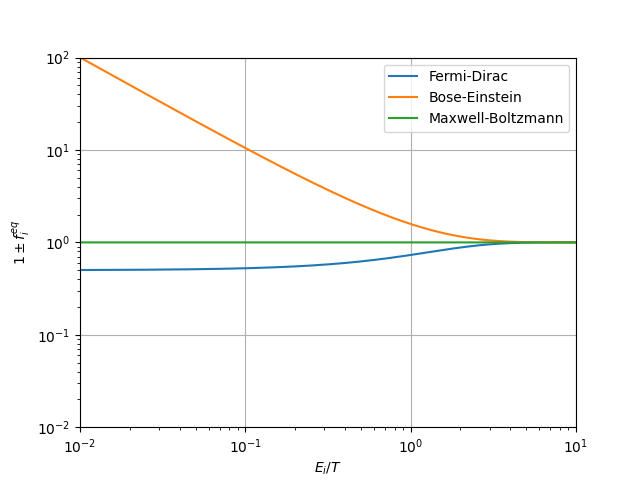
\includegraphics[width=0.7\linewidth]{graphs/1+-fi}
	\caption{Dependance of $1\pm f_i$ with $E_i/T$.}
	\label{fig:1-fi}
\end{figure}

For the process of annihilation ($1+2 \leftrightarrow 3+4$), where the particles $3$ and $4$ are in thermal equilibrium, and considering the conservation of energy ($E_1+E_2=E_3+E_4$) we check that
\begin{equation}
	f_3^{eq}f_4^{eq}=e^{-(E_3+E_4)/T}=e^{-(E_1+E_2)/T}=f_1^{eq}f_2^{eq}\,.
\end{equation}

The cross section for a process $1+2\rightarrow3+4$ is 
\begin{equation}
	\label{crosssection}
	\sigma=\frac{S_{12}S_{34}}{4\sqrt{(\mathcal{P}_1\cdot\mathcal{P}_2)^2-(m_1m_2)^2}}\int (2\pi)^4\delta^4(\mathcal{P}_1+\mathcal{P}_2-\mathcal{P}_3-\mathcal{P}_4)\frac{|M|^2}{g_1g_2}\frac{d\Pi_3d\Pi_4}{g_3g_4}\,.
\end{equation}

Using the \autoref{eqn:3.1}, for the number density as
\begin{equation}
	\label{dni}
	dn_i=\frac{g_i}{(2\pi)^3}\frac{d\vec{p}_i}{2E_i}\,,
\end{equation}
and the \autoref{crosssection}, we can simplify the \autoref{eqn:3.38} to
\begin{equation}
	\label{3.45}
	\int C[f_1] d\Pi_1 = -\int \sigma v_{\textrm{M{\o}ller}}\left[dn_1dn_2-dn_1^{eq}dn_2^{eq}\right]\,,
\end{equation}
where $v_{\textrm{M{\o}ller}}$, is the M{\o}ller velocity, and is defined as
\begin{equation}
	\label{vmoller}
	v_{\textrm{M{\o}ller}}=\frac{\sqrt{(\mathcal{P}_1\cdot\mathcal{P}_2)^2-(m_1m_2)^2}}{E_1E_2}\,,
\end{equation}
the M{\o}ller velocity turns the product $v_{\textrm{M{\o}ller}}n_1n_2$ invariant under Lorentz\,, \cite{GONDOLO}.

Therefore we can write our \autoref{3.45}, as
\begin{equation}
	\label{eqn:3.47}
	\frac{g_1}{(2\pi)^3}\int \frac{d\vec{p}_1}{2E_1}C[f_1]=-\langle\sigma v_{\textrm{M{\o}ller}}\rangle[n_1n_2-n_1^{eq}n_2^{eq}]\,,
\end{equation}
where the thermal averaged cross section is defined as
\begin{equation}
	\label{tacs}
	\langle \sigma v_{\textrm{M{\o}ller}}\rangle=\dfrac{\mathlarger{\int} (\sigma v_{\textrm{M{\o}ller}})dn_1^{eq}dn_2^{eq}}{\mathlarger{\int} dn_1^{eq}dn_2^{eq}}\,,
\end{equation}
for simplicity we are going to denote the thermal averaged cross-section as $\langle\sigma v\rangle$.

Let's take a look at the number density of the particles coupled with the thermal bath, knowing these particles will follow the Maxwell-Boltzmann distribution, with $\mu=0$, we can write the \autoref{eqn:3.17} as
\begin{equation}
	\label{nthermalbath}
	n=\frac{g}{(2\pi)^3}4\pi\int_{m}^{\infty} E\sqrt{E^2-m^2}e^{-E/T}dE\,,
\end{equation} 
where we use $E^2=|\vec{p}|^2+m^2$ and spherical symmetry of the momentum, $d\vec{p}=4\pi E \sqrt{E^2-m^2}dE$. The inferior limit comes from the minimum energy possible of the particle, which is its rest mass.

Integrating by parts the \autoref{nthermalbath}, we get
\begin{equation}
	n=\frac{g}{(2\pi)^3}4\pi\left(\frac{1}{3}\left[(E^2-m^2)^{3/2}e^{-E/T}\right]_m^\infty+\frac{1}{3T}\int_{m}^{\infty}(E^2-m^2)^{3/2}e^{-E/T}dE\right)\,,
\end{equation}
we can easily see that the left side gives zero, and the right side can be related to the Bessel function, which is defined as
\begin{equation}
	 \label{bessel}
	 K_\alpha(z)=\frac{\sqrt{\pi}}{\Gamma(\alpha+1/2)}\left(\frac{z}{2}\right)^\alpha\int_{1}^{\infty}(x^2-1)^{\alpha-1/2}e^{-zx}dx\,,
\end{equation}
and so making $x=E/m$ and $z=m/T$, and knowing that $\Gamma(5/2)=3\sqrt{\pi}/4$, we get
\begin{equation}
	\label{nbessel}
	n=\frac{g}{2\pi^2}m^2TK_2(m/T)\,.
\end{equation}

From Equations (\ref{tacs}) and (\ref{dni}) we can see that

\begin{equation}
	\label{eqn:3.52}
	\langle \sigma v_{\textrm{M{\o}ller}}\rangle=\dfrac{\mathlarger{\int}(\sigma v_{\textrm{M{\o}ller}})e^{-E_1/T}e^{-E_2/T}d^3p_1d^3p_2}{\mathlarger{\int} e^{-E_1/T}e^{-E_2/T}d^3p_1d^3p_2}	\,.
\end{equation}

Let's now consider that the particle 1 is equal to the particle 2, as it will be the main scope of this project.
Following the \autoref{nbessel}, it's easy to see that the denominator of the \autoref{eqn:3.52} will be
\begin{equation}
	\label{3.53}
	\int e^{-E_1/T}e^{-E_2/T}d\vec{p}_1d\vec{p}_2=(4\pi m^2 T K_2(m/T))^2\,,
\end{equation}
where $m=m_1=m_2$

Let's now look at the numerator of the \autoref{eqn:3.52}, using spherical symmetry ($d\vec{p}_i=4\pi E_i |\vec{p}_i| dE_i$) we can see that
\begin{equation}
	\label{volume1}
	d^3p_1d^3p_2=4\pi E_1 |\vec{p}_1| 4\pi E_2 |\vec{p}_2|  \frac{1}{2}dE_1dE_2d\cos(\theta)\,,
\end{equation}
where $\theta$ is the angle between $\vec{p}_1$ and $\vec{p}_2$, notice that the term $d\cos(\theta)/2$ is invariant under integration, for simplicity we are going to make a few changes of variables
\begin{equation}
	\left\{\begin{array}{l}
			E_+=E_1+E_2 \\
			E_-=E_1-E_2 \\
			s=2m^2+2E_1E_2-2|\vec{p}_1||\vec{p}_2|\cos(\theta)
	\end{array} \right.	\Leftrightarrow
	\left\{\begin{array}{l}
		E_1=\frac{E_++E_-}{2} \\
		E_2=\frac{E_+-E_-}{2} \\
		\cos(\theta)=\dfrac{-s+2m^2+2(E_+^2-E_-^2)}{2|\vec{p}_1||\vec{p}_2|}
	\end{array} \right.\,,
\end{equation}
where $s=\left(\mathcal{P}_1+\mathcal{P}_2\right)^2$ is a Mandelstam variable \cite{otto}.

Using the Jacobian matrix we can see that
\begin{align}
	\begin{array}{ll}
		dE_1dE_2d\cos(\theta)
		=&\left| 
		\begin{array}{lll} 
			\frac{\partial E_1}{\partial E_+} & \frac{\partial E_1}{\partial E_-} & \frac{\partial E_1}{\partial s}\\
			\frac{\partial E_2}{\partial E_+} & \frac{\partial E_2}{\partial E_-} & \frac{\partial E_2}{\partial s}\\
			\frac{\partial \cos(\theta)}{\partial E_+} & \frac{\partial \cos(\theta)}{\partial E_-} & \frac{\partial \cos(\theta)}{\partial s}
		\end{array} \right|dE_+dE_-ds \\ [15pt]
	&= (2|\vec{p}_1||\vec{p}_2|)^{-1}dE_+dE_-ds\,.
	\end{array}
\end{align}


The volume element, in \autoref{volume1} becomes

\begin{equation}
	\label{volume2}
	d^3p_1d^3p_2=2\pi^2E_1E_2dE_+dE_-ds\,,
\end{equation}
and the integration limits, from $E_1\geq m_1$, $E_2\geq m_2$, $|\cos(\theta)|\leq 1$, become
\begin{equation}
	\left\{
	\begin{array}{l}
		s \geq 4m^2 \\
		E_+\geq \sqrt{s} \\
		|E_-| \leq \sqrt{1-\frac{4m^2}{s}} \sqrt{E_+^2-s}
	\end{array}
	\right.\,.
\end{equation}

Therefore, the numerator from \autoref{eqn:3.52} will be

\begin{equation}
	\int (\sigma v_{\textrm{M{\o}ller}})e^{-E_1/T}e^{-E_2/T}d^3p_1d^3p_2=2\pi^2\int dE_- \int dE_+ \int \sigma v_{\textrm{M{\o}ller}} E_1 E_2 e^{-E_+/T}ds\,,
\end{equation}
then from the definition of $v_{\textrm{M{\o}ller}}$ in \autoref{vmoller},

\begin{align}
	\label{3.60}
	\begin{array}{ll}
		\mathlarger{\int} (\sigma v_{\textrm{M{\o}ller}})e^{-E_1/T}e^{-E_2/T}d^3p_1d^3p_2&=
		4\pi^2 \mathlarger{\int} \sigma G \sqrt{1-\frac{4m^2}{s}}ds \mathlarger{\int} e^{E_+/T}\sqrt{E_+^2-s}dE_+ \\ [15pt]
		&= 2\pi^2 T \mathlarger{\int} \sigma (s-4m^2) \sqrt{s}K_1(\sqrt{s}/T)ds\,,
	\end{array}
\end{align}
where we define $G \equiv v_{\textrm{M{\o}ller}}E_1E_2=\frac{1}{2}\sqrt{s(s-4m^2)}$ and we use the Bessel function, in \autoref{bessel}, with $\alpha=1$.

Let us use the Equations (\ref{3.53}) and (\ref{3.60}), to simplify the thermal averaged cross section, in \autoref{tacs}, to
\begin{equation}
	\label{sigmav}
	\langle \sigma v_{\textrm{M{\o}ller}}\rangle=\frac{1}{8m^4TK_2^2(m/T)}\int_{4m^2}^{\infty}\sigma(s-4m^2)\sqrt{s}K_1(\sqrt{s}/T)ds\,.
\end{equation}

